% Name: Flowchart symbols
% Description: A key to the standard flowchart shapes: terminal, process, decision, input and output, predefined process, document, database, and connector.
% Tags: flowchart, symbols, legend, ISO 5807

\usetikzlibrary{shapes.geometric, shapes.misc}

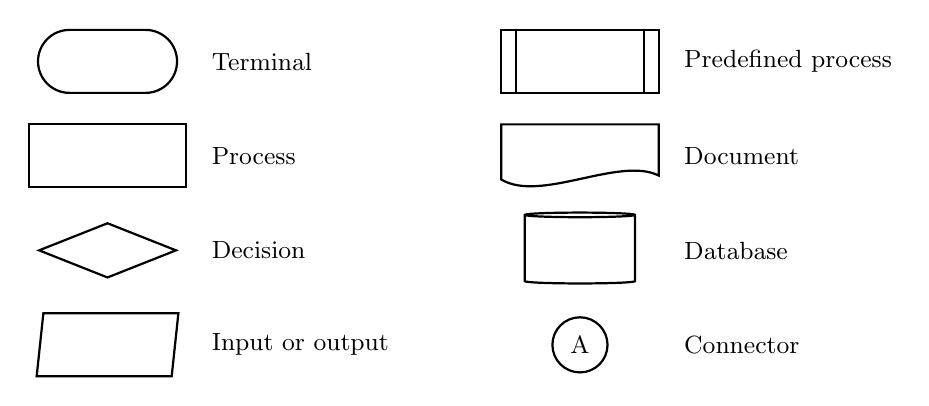
\begin{tikzpicture}[
  every node/.style={font=\small},
  sym/.style={draw, thick, minimum width=20mm, minimum height=8mm},
  caption/.style={anchor=west},
]
  \node[sym, rounded rectangle] (a) at (0,0) {};
  \node[sym] (b) at (0,-1.2) {};
  \node[sym, diamond, aspect=2.5, minimum width=0pt, minimum height=0pt, inner sep=2.5mm] (c) at (0,-2.4) {};
  \node[sym, trapezium, trapezium left angle=70, trapezium right angle=110, trapezium stretches body, minimum width=18mm] (d) at (0,-3.6) {};
  \node[sym] (e) at (6,0) {};
  \draw[thick] ([xshift=2mm]e.north west) -- ([xshift=2mm]e.south west) ([xshift=-2mm]e.north east) -- ([xshift=-2mm]e.south east);
  \draw[thick] (5,-0.8) -- (7,-0.8) -- (7,-1.45) .. controls (6.5,-1.2) and (5.5,-1.8) .. (5,-1.5) -- cycle;
  \node[sym, cylinder, shape border rotate=90, aspect=0.25, minimum width=14mm, minimum height=9mm] (g) at (6,-2.4) {};
  \node[draw, thick, circle, minimum size=7mm] (h) at (6,-3.6) {A};

  \foreach \y/\left/\right in {0/Terminal/Predefined process, -1.2/Process/Document, -2.4/Decision/Database, -3.6/Input or output/Connector} {
    \node[caption] at (1.2,\y) {\left};
    \node[caption] at (7.2,\y) {\right};
  }
\end{tikzpicture}
